% !TEX encoding = UTF-8
% !TEX TS-program = pdflatex
% !TEX root = ../Tesi.tex
% !TEX spellcheck = it-IT

%************************************************
\chapter{CUDA - Compute Unified Device Architecture}
\label{cap:CUDA}
%************************************************

\section{Introduzione}
Quasi nove anni fa, nel Novembre 2006  la \textbf{NVIDIA Corporation} ha
rilasciato CUDA, una piattaforma (hardware e software insieme) che permettono di
utilizzare linguaggi di programmazione ad alto livello (Ad es. \textbf{C},
\textbf{C++}, \textbf{Java}) per implementare codice parallelo per risolvere
problemi molto complessi a livello computazionale in una maniera efficiente
rispetto alle normali CPU.

\begin{figure}[h] 
\centering 
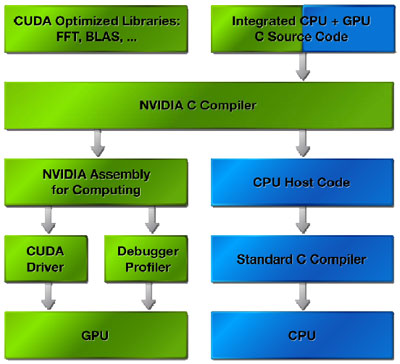
\includegraphics[width=0.5\columnwidth]{Immagini/cuda_compiler} 
\caption[Compilatore NVCC]{Struttura di Nvidia C Compiler.\\}
\label{fig:cuda_compiler} 
\end{figure}

CUDA � molto utilizzato poich� � un sistema completo e anche molto semplice da
capire ed utilizzare. Sopratutto quest'ultimo particolare � di importante
rilevanza, dato che attualmente le alternative a CUDA, come OpenCL, risultano
essere molto pi� complesse a livello implementativo e di leggibilit� del
codice.
Come illustrato in figura \ref{fig:cuda_compiler}, NVIDIA fornisce un
compilatore capace di riconoscere le istruzioni CUDAma l'implementazione di un
programma parallelo avviene utilizzando codice sorgente sia per CPU che per GPU.
Il compilatore NVIDIA C (\textit{nvcc}) dunque, identifica il tipo di istruzione
richiamando i compilatori di riferimento gestendo cos� questa convivenza.
  
\section{Architettura hardware}

Oggi sul mercato delle schede video possiamo trovare innumerevoli tipi di
device, e i computer moderni referibilmente posseggono una scheda video
dedicata. In particolare la \textbf{Nvidia Corporation} ha creato anche diverse
architetture hardware per soddisfare ogni tipo di richiesta. Quelle conosciute
sono le architetture \textbf{Kepler}, \textbf{Fermi} e \textbf{Tesla}.
L'architettura Kepler � quella pi� utilizzata nei computer in commercio con
scheda grafica NVIDIA.

 In generale, le architetture GPU NVIDIA, sono composte da un array di
 \textit{Streaming Multiprocessors (SMs)}. Lo Streaming Multiprocessors �
 progettato per eseguire centinaia di threads in parallelo e contiene un
 determinato numero di Streaming Processors (SP). Gli Streaming processors sono
 anche chiamati \textit{CUDA cores} e il loro numero dipende dalla capacit� del
 device installato.
 
 \subsection{Compute capability}
Ogni device possiede un \textit{revision number} che possiamo definire come la
\textbf{compute capability} del device, e determina l'insieme di funzionalit�
che possono essere usate nell'implementazione di codice parallelo in CUDA.
La compute capability � definita dal pi� alto numero di revision number e il
minor numero di revision number. Nel caso in cui devices diversi abbiano il pi�
alto revision number posseggono la stessa architettura. Il pi� alto numero di
revision number per le architetture Kepler � 3, per i devices basati su
un'architettura Fermi � 2, mentre per i device con architettura Tesla 1. Il
numero minore di revision number invece, corrisponde al miglioramento del core
dell'architettura che spesso porta a nuove funzionalit� da poter utilizzare
tramite le API fornite appunto da NVIDIA.

\subsection{Architettura Kepler}
L'architettura Kepler � stata progettata e successivamente lanciata nel 2010
insieme all'architettura Fermi. La prima GPU basata sull'architettura Kepler si
chiamava \''GK104\'' in cui ogni unit� interna � stata progettata ai fini di
avere la miglior performance per watt (perf/watt). Alcuni esperti hanno
affermato che la GK104 Kepler � la GPU pi� potente per la computazione e il
rendering grafico dei videogames.

Inizialmente la GPU utilizzata per questo lavoro di tesi � stata la NVIDIA
GeForce GT 750M basata anch'essa su un architettura Kepler. Il core in
particolare � il \''GK107\'' che offre due shader di blocchi, chiamati
\textbf{SMX}, ognuno dei quali ha 192 shaders per un totale di 384 shader cores
con una velocit� di 967 MHz.

\begin{figure}[h] 
\centering 
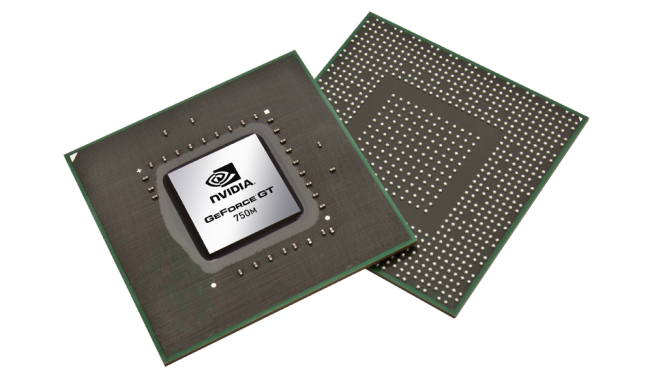
\includegraphics[width=0.5\columnwidth]{Immagini/gt750m} 
\caption[GT 750M]{La scheda video NVIDIA GT 750-M.\\}
\label{fig:gt750m} 
\end{figure} 

\section{Interfaccia di programmazione}
CUDA � un sistema progettato per elaborare codice parallelo per le GPU Nvidia.
Essa fornisce al programmatore un insieme di astrazioni facilmente
comprensibili, consentendo cos� di \cite{SCIARA:2001}

\subsection{Host e Device}
\subsection{I kernel}
\subsection{La memoria}
\subsection{Parallelismo dinamico}

\section{Tools di sviluppo}
\subsection{Nsight}
\subsection{Visual Profiler}